\subsection{Quantifying Differences Between Mutants}

The raw data on the mutant roots presented in Figure \ref{fig:mutant-sizes} is in units of cell number versus cell length. The data was gathered from approximately $30$ cell columns per mutant, with each column originating from a different plant. We transformed this data into units of time and length using the following procedure. First, we made the assumption that cells are perfect cylinders, so that their cross sectional area is equal to their length multiplied by their diameter. Then, we assumed that the diameter of each cell is identical, and prescribed a suitably chosen diameter $d = 10\um$ based on experimental data (\cite{goh2023}). To convert cell number to position we took the cumulative sum of the cell lengths over each cell column. Missing data was filled in using the average length for that cell number and mutant. The results of this data preprocessing is shown in Figure \ref{sfig:data-trichoblast}.

\begin{supplementaryfigure}
    \centering
    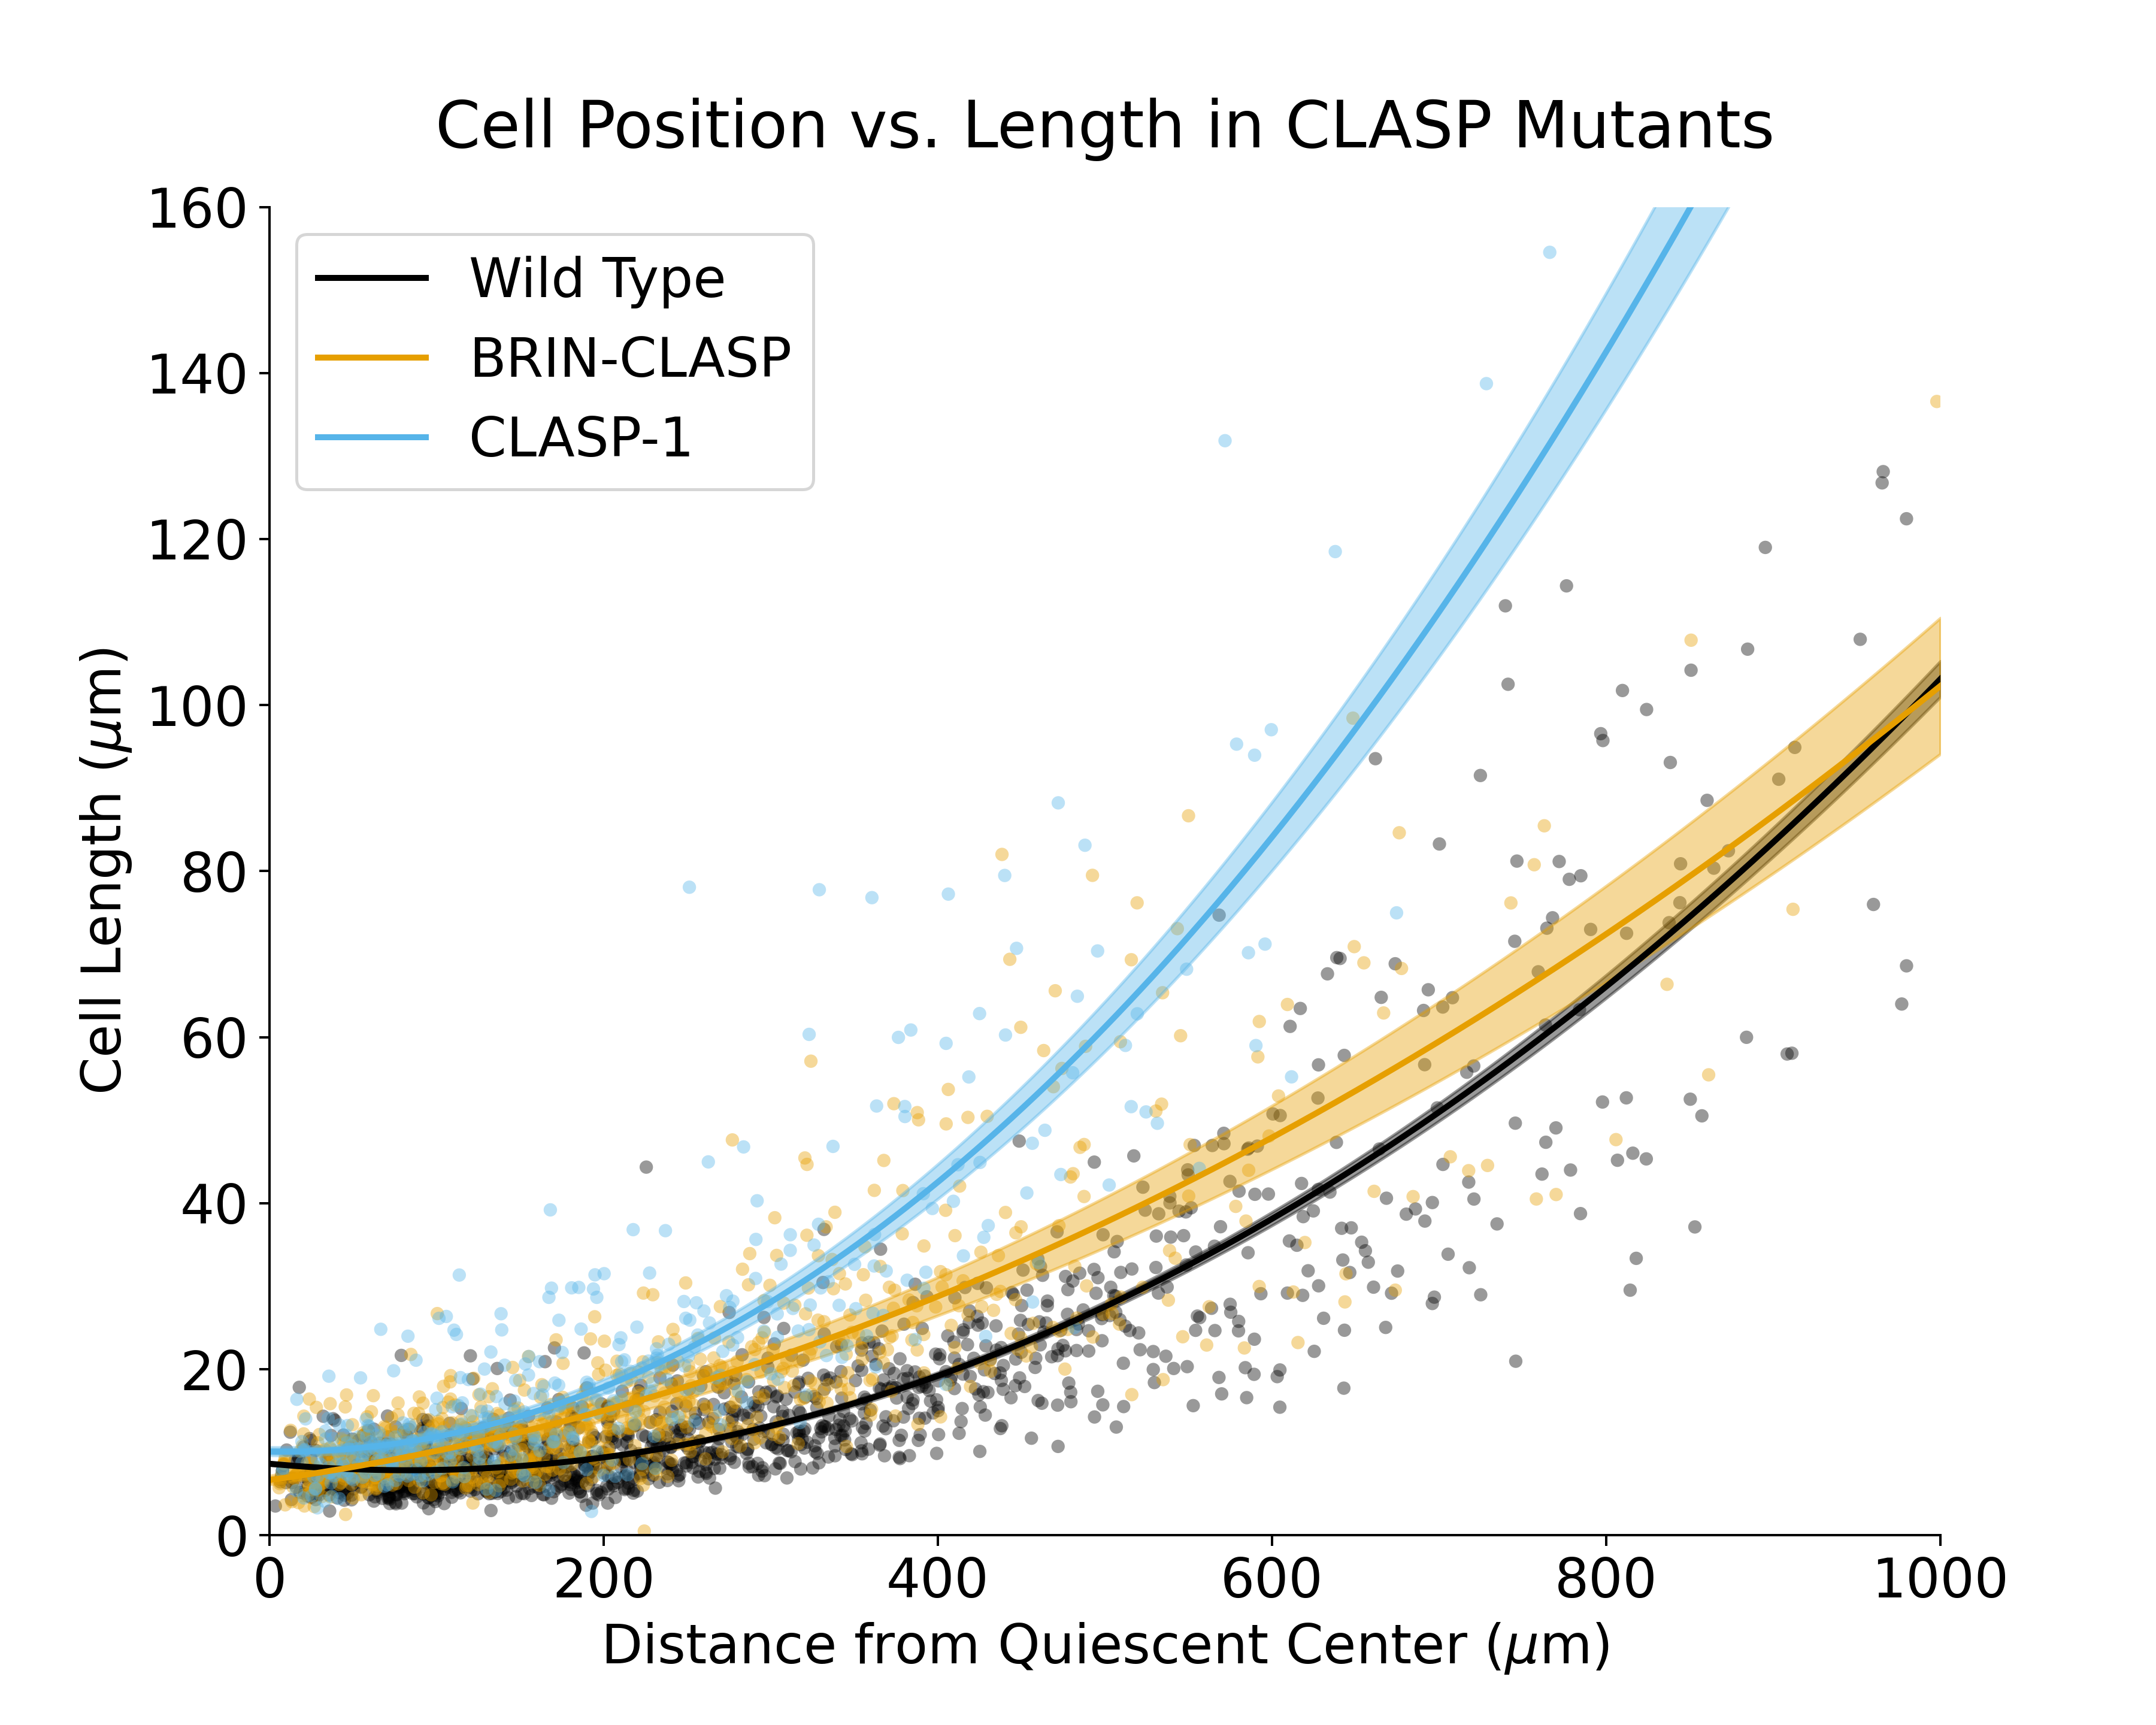
\includegraphics[width=13cm]{img/data-trichoblast.png}
    \caption{Plot of cell lengths from trichoblast cells in wild type, CLASP-1, and BRIN-CLASP roots. The line of best fit is an exponential function of the form $A + Be^{Cx}$. Wild type cells are on average the shortest, followed closely by BRIN-CLASP. CLASP-1 cells are significantly longer, especially in the proximal regions of the root. There is a large amount of variance in the data, especially at higher positions.}
    \label{sfig:data-trichoblast}
\end{supplementaryfigure}

\medskip

We wish to quantify the differences between the mutants in order to confirm that their behaviour is indeed different from the wild type. To do this, we computed the relative error of each data point from the line of best fit for the wild type cells. The distribution of these errors is shown in Figure \ref{sfig:trichoblast-distribution}. Cells in the BRIN-CLASP root have a mean error of $+41\%$ from the wild type average, while cells in the CLASP-1 root have a mean error of $+80.9\%$. This suggests a significant effect size for the various mutations. Additionally, the mutations were statistically significant with $p$-values less than $10^{-20}$, which provides further evidence that the mutants are exhibiting different behaviour.

\begin{supplementaryfigure}
    \centering
    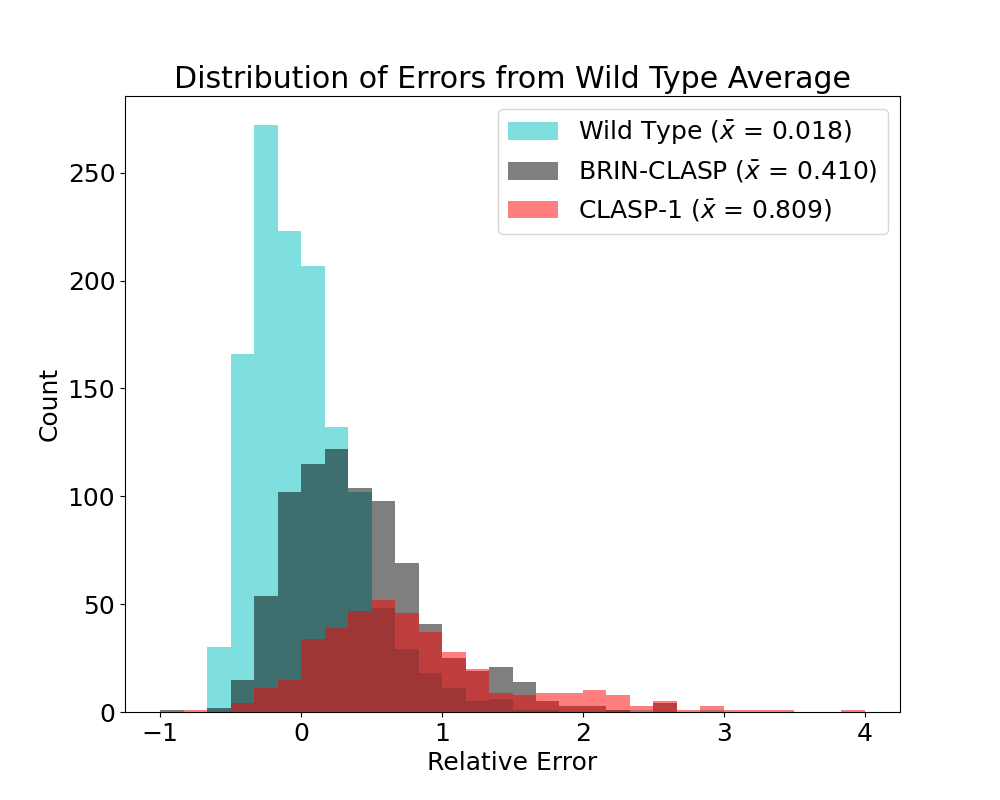
\includegraphics[width=13cm]{img/trichoblast-distribution.png}
    \caption{Distribution of errors from the wild type average presented in Figure \ref{sfig:data-trichoblast}. The mean error of the BRIN-CLASP and CLASP-1 mutants are clearly positive, which suggests that on average, the mutants have longer cells compared to the wild type. }
    \label{sfig:trichoblast-distribution}
\end{supplementaryfigure}


